\chapter{Introduction}
\label{chap:chap0}

While the term \emph{robotics} was first coined by Isaac Asimov some
seventy years ago, and while the first industrial robots were
developed in 1961, the description of automaton mechanisms can
be dated back to the tenth century B.C., which is a proof of Man's
long-time fascination with robots. The first robots had limited
capabilities, mainly focused on moving some of their limbs in order to
\emph{act} on their environment or simply to entertain. Starting from
the middle of the twentieth century, technological advances in
electronics allowed the creation of sensors which allowed robots to
\emph{perceive} their surroundings (including their own body), i.e. to
build a useful representation of them. Finally, thanks to the
breakthroughs in the Computer Science and Mathematics fields, the
means to \emph{decide} how to act based on perception were given to
robots (and roboticists too!). This decision process is known as
\emph{planning}.

\section{Anthropomorphic Systems in Robotics}

Anthropomorphic systems can be described as systems which are made to
look like humans with respect to their mechanical structure and their
abilities. In robotics, they usually have similar perception systems,
such as visual sensors in the head, tactile and inertial
sensors. Also, they usually have two arms and more importantly two
legs, which sets them apart from wheeled robots. These features are
such that it is very complex to implement a perception-planning-action
on anthropomorphic systems (or humanoid robots).

So why do we bother designing and studying anthropomorphic systems?
Simply because it is fun! As the reader may still be skeptical with
respect to this argument, there are luckily many applications for
humanoids robotics. First of all, as humanoid robots are made to look
like humans, they have similar abilities that can allow them to walk,
run, jump, climb, write, carve, manipulate, etc. There are of course
highly specialized robots that can achieve each one of those tasks,
but very few exhibit such a high versatility. Also, we are witnessing
a shift from industrial robotics to personal robotics. Humanoid robots
can have access to the same environments as humans, and they are made
to look like them and to be easily accepted: they can therefore be
used as companions, assistants, guides, teachers, etc in various
situations.

From a research point of view, anthropomorphic systems are very
interesting as they give researchers the means to devise new
algorithms to control them and make them walk and manipulate objects
without loosing their balance, allowing the generation of human-like
motions. Conversely, humanoid robots are perfect tools for
neuroscientists to understand human motion and perception, as well as
the invariants behind them; for instance, moving certain actuators
while keeping others at a fixed position is very easy in robotics, and
this allows decoupling different behaviors in order to observe them
more clearly. Humanoid robots also tend to be more cooperative (so
far) than humans or monkeys when it comes to accomplishing tedious and
repetitive tasks during experiments.

\begin{figure}
  \centering
      {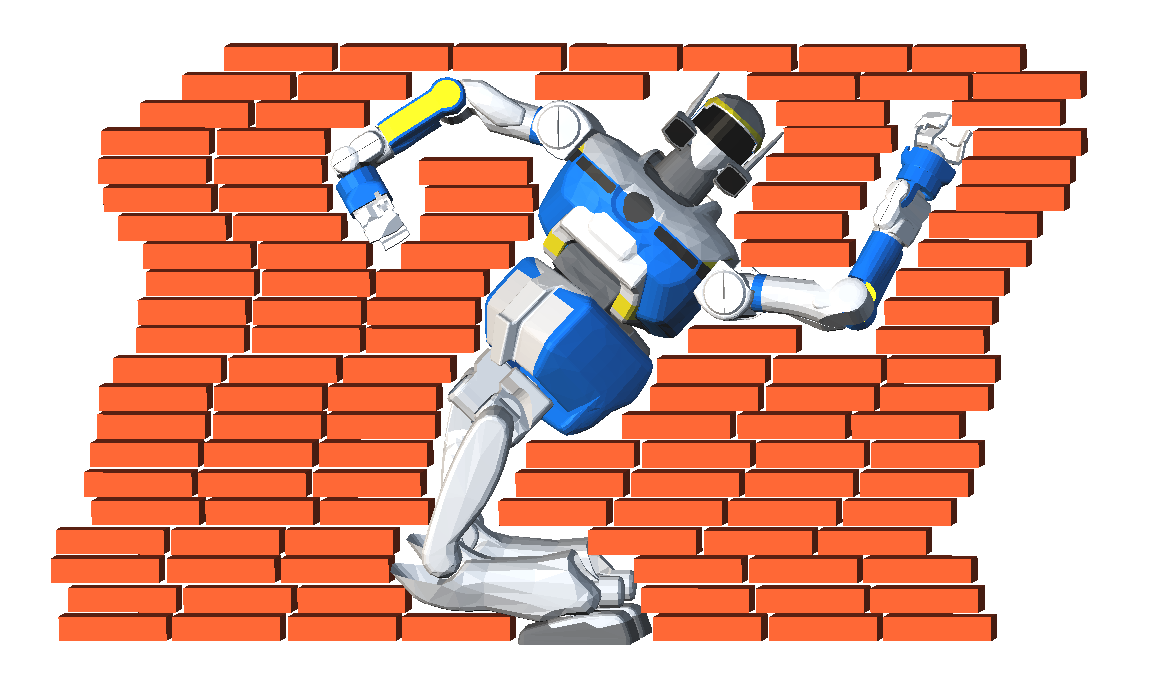
\includegraphics[width = 0.7\linewidth]
        {src/chap0-introduction/hrp2-brick-wall.png}}
      \caption{The human-like mechanical structure of humanoid robots
        enables them to accomplish complex tasks, such as avoiding
        obstacles in constrained environments.}
      \label{fig:chap0-hrp2-brick-wall}
\end{figure}

In this thesis, we focus on developing new algorithmic tools for
\emph{planning optimal motions for anthropomorphic systems}, as well
as applying them on humanoid robots.

\section{Problem Statement}

The problem of motion planning for anthropomorphic systems can be
defined as the following: given a starting configuration, say a
position and posture, we would like an anthropomorphic system, say a
humanoid robot or a digital actor, to reach a goal configuration if it
is possible. Obviously such a system cannot move instantaneously, so
it will have to travel continuously in the environment surrounding it
to reach its goal. The environment will usually not be empty, as it
will contain at least the floor that supports the system. It might
also contain moving or static entities with which we do not want the
system to collide in order to avoid damaging either the entities, the
system, or both. Additionally, we want to avoid self-collisions
between the different limbs of the system. Finally, as anthropomorphic
systems rely on making and breaking contact with their environment in
order to move, great care must be given to make sure the system can
realize the required motions and does not fall. This requires a good
definition of a system \emph{balance} and the means to ensure
it. Therefore, finding a solution to the problem of humanoid walk
planning consists in finding a continuous motion connecting the start
configuration to the goal configuration, such that the anthropomorphic
system is never in collision with the environment or itself when
executing this motion, and such that it is always balanced.

While the found solution is guaranteed to be collision-free, we still
know nothing about its quality. In the case of anthropomorphic system
motion, the notion of quality can be linked to how close a motion is
to real human motion, i.e. one which a human being would have made if
he was put in the same conditions. Obtaining high-quality motions is
desirable since humanoid robots are bound to move in man-made
environments such as homes, offices, and factories and because it
could help them blend in among humans more seamlessly. Subsequently,
we would like to impose additional constraints on the motion planning
problem in order to find motions that are both collision-free and
optimal with respect to a certain cost measure. We refer to this
problem by the name of optimal motion planning.

\begin{figure}[h!]
  \centering
      {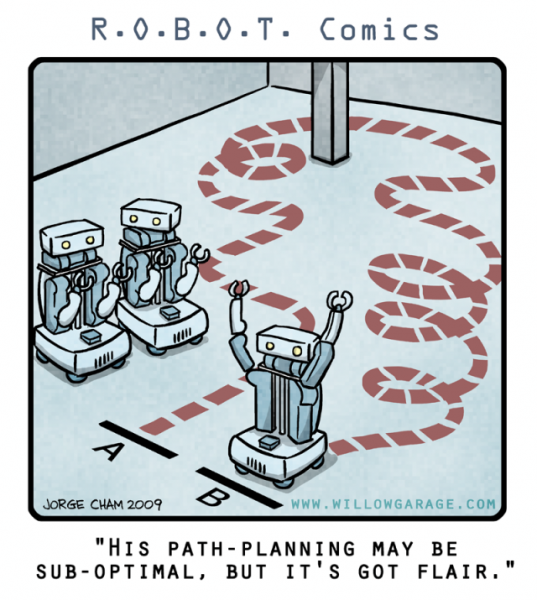
\includegraphics[width = 0.6\linewidth]
        {src/chap0-introduction/optimal-motion-planning.png}}
      \caption{A robot solves a motion planning problem. The solution
        is collision-free, but obviously the robot can do much better
        (Jorge Cham, PhD Comics).}
      \label{fig:chap0-optimal-motion-planning}
\end{figure}

\section{Contributions}

\emph{The first contribution} of this thesis is a heuristic and
efficient optimization method that takes as input a path computed for
the robot bounding box, and produces a path where a discrete set of
configurations is reoriented using an A* search algorithm. The
resulting trajectory is realistic and time-optimal. This method is
validated on various scenarios.

\emph{The second contribution} is a whole-body motion planner for
humanoid robots which computes collision-free walking trajectories,
based on exact models of both robot and environment. It is used to
solve manipulation tasks that may require walking. The first stage of
our algorithm uses a sampling-based constrained motion planner and
computes a collision-free statically balanced path for a robot which
can be fixed or sliding on the ground. The formal proof that dynamic
walking makes humanoid robots small-space controllable is then
established; this directly implies that this first path can always be
approximated by a dynamically balanced, collision-free walking
trajectory. This well-grounded method is implemented and the results
are validated on several environments.

A new framework for optimal motion planning is proposed as a
\emph{third contribution}. Given a humanoid robot geometric and
dynamic model, an exact model of the environment, start and end
configurations, and a robot contact stance, we first plan a
collision-free statically balanced path that satisfies all kinematic
constraints. We convert the path to an initial trajectory using a
suitable time parametrization, and we then optimize it to generate a
locally-optimal collision-free dynamically-balanced trajectory. This
involves both finding a new time parametrization for the trajectory,
and reshaping the path in a geometrical sense; thus, it is not simply
a problem of optimal path tracking. In order to ensure
(self-)collision avoidance during the optimization process, we choose
to model distance constraints using bounding capsules around the robot
exact body geometries. We provide an automatic bounding capsule
generation tool; it relies on a numerical optimization problem
formulation that allows us to find the minimum-volume capsules around
bodies which are modeled by polyhedra. The capsules allow us then to
enforce collision-avoidance constraints between the robot, the
obstacles and itself.

\section{Outline of This Thesis}

The thesis is organized by contribution order, and the related work is
explained when needed. Chapter \ref{chap:path-optim} describes the
path optimization method for humanoid walk planning. Chapter
\ref{chap:wholebody-planning} deals with the second contribution,
namely whole body motion planning and the associated small-space
controllability proof. Finally, the optimal motion planning framework
and the automatic bounding capsule generator are detailed in Chapter
\ref{chap:optimal-motion-planning}.

\section{Publications in This Thesis}

\subsection*{Journal}

\begin{itemize}
\item S\'ebastien Dalibard, Antonio El Khoury, Florent Lamiraux,
  Alireza Nakhaei, Michel Ta\"ix and Jean-Paul
  Laumond. \textbf{Dynamic Walking and Whole-Body Motion Planning for
    Humanoid Robots: an Integrated Approach,} \textit{International
    Journal of Robotics Research, 2013.}
\end{itemize}

\subsection*{Peer-Reviewed International Conferences}
\begin{itemize}
\item Antonio El Khoury, Michel Ta\"ix and Florent
  Lamiraux. \textbf{Path Optimization for Humanoid Walk Planning: an
    Efficient Approach,} \textit{International Conference on
    Informatics in Control, Automation and Robotics, 2011.}

\item S\'ebastien Dalibard, Antonio El Khoury, Florent Lamiraux,
  Michel Ta\"ix and Jean-Paul Laumond. \textbf{Small-Space
    Controllability of a Walking Humanoid Robot,} \textit{IEEE
    International Conference on Humanoid Robots, 2011.}

\item Antonio El Khoury, Florent Lamiraux and Michel
  Ta\"ix. \textbf{Optimal Motion Planning for Humanoid Robots,}
  \textit{IEEE International Conference on Robotics and Automation,
    2013.}
\end{itemize}

\section{Videos of Simulations and Experiments}

%%FIXME%%

A permanent link to videos of experiments realized in this thesis will
be added here.

\section{Software Contributions in This Thesis}

Several open-source software packages were created or extended
throughout this thesis. Some of them include:

\begin{itemize}
  \item \textit{kws-hash-optimizer}: a package for an efficient path
    optimization method, which is described in Chapter 1.
  \item \textit{hpp-wholebody-step-planner}: a package for humanoid whole-body
    motion planning. It implements the algorithm that is presented in
    Chapter 2 of this thesis.
  \item \textit{roboptim-capsule}: an automated bounding capsule generator over
    polyhedrons. It is based on an optimization formulation, which is
    presented in Chapter 3.
  \item \textit{MetaPOD} (Meta-Programming Optimized Dynamics): a
    template-based C++ implementation of \cite{feat08}. It is used in
    the optimal control formulation which is described in Chapter 3.
\end{itemize}
